\documentclass[11pt,a4paper]{article}
\usepackage[T1]{fontenc}
\usepackage[utf8]{inputenc}
\usepackage{lmodern,microtype}
\usepackage[margin=24mm,headheight=14pt]{geometry}
\usepackage{amsmath,amssymb,mathtools,bm}
\usepackage{graphicx,booktabs,array,enumitem}
\usepackage{xcolor,tikz}
\usetikzlibrary{arrows.meta,positioning}
\usepackage{fancyhdr}
\usepackage[numbers,sort&compress]{natbib}
\definecolor{ink}{HTML}{233346}
\definecolor{accent}{HTML}{176B82}
\definecolor{wash}{HTML}{EAF3F6}
\usepackage[colorlinks=true,linkcolor=accent,citecolor=accent,urlcolor=accent]{hyperref}
\pagestyle{fancy}\fancyhf{}
\fancyhead[L]{\small\textcolor{ink}{HAC 2026 \;|\; OT convex reconstruction}}
\fancyhead[R]{\small Method note}
\fancyfoot[C]{\small\thepage}
\renewcommand{\headrulewidth}{0.3pt}
\setlength{\parindent}{0pt}
\setlength{\parskip}{6pt}
\setlist{nosep,leftmargin=1.5em}
\setlength{\emergencystretch}{2em}
\newcommand{\R}{\mathbb{R}}
\newcommand{\sphere}{\mathbb{S}^{2}}
\newcommand{\norm}[1]{\left\lVert#1\right\rVert}
\newcommand{\OT}{\operatorname{OT}}
\newcommand{\diag}{\operatorname{diag}}
\newcommand{\cof}{\operatorname{cof}}
\hypersetup{pdftitle={Optimal-transport convex reconstruction for HAC 2026},pdfsubject={Reproducible method note}}
\begin{document}
\thispagestyle{empty}
{\color{accent}\small HELSINKI ASTEROID CHALLENGE 2026}\par
\vspace{5pt}
{\LARGE\bfseries Optimal-transport convex reconstruction}\par
\vspace{3pt}
{\large From changing brightness to a closed three-dimensional shape}\par
\vspace{5pt}
{\small Method note \hfill 7 September 2026}
\vspace{12pt}

\textbf{The central idea.} Instead of moving thousands of mesh vertices while fitting the data, we first estimate how much surface area faces each direction. Optimal transport supplies a prior on this directional distribution and helps compress it into a manageable set of facets. A separate geometric solver then finds a convex polyhedron with those facet normals and areas.

The input is a collection of \emph{lightcurves}: total image brightness measured as an object completes a rotation. The camera does not resolve the object's three-dimensional surface. Shape information comes from how brightness changes with rotation and viewing geometry. This is the setting of classical convex lightcurve inversion~\cite{kaasalainen2001}; our particular representation, regularization, and export checks are described below.

\begin{figure}[h]
\centering\resizebox{\linewidth}{!}{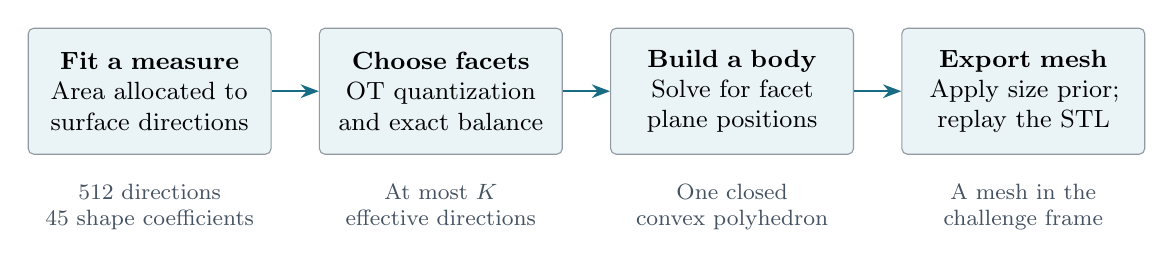
\begin{tikzpicture}[>=Stealth,node distance=0.6cm,
 block/.style={draw=ink!50,rounded corners=2pt,fill=wash,text width=2.85cm,minimum height=1.6cm,align=center,font=\small},
 smallnote/.style={align=center,font=\footnotesize,text=ink!85}]
\node[block] (a) {\textbf{Fit a measure}\\Area allocated to\\surface directions};
\node[block,right=of a] (b) {\textbf{Choose facets}\\OT quantization\\and exact balance};
\node[block,right=of b] (c) {\textbf{Build a body}\\Solve for facet\\plane positions};
\node[block,right=of c] (d) {\textbf{Export mesh}\\Apply size prior;\\replay the STL};
\draw[->,thick,color=accent] (a)--(b);
\draw[->,thick,color=accent] (b)--(c);
\draw[->,thick,color=accent] (c)--(d);
\node[smallnote,below=0.25cm of a] {512 directions\\45 shape coefficients};
\node[smallnote,below=0.25cm of b] {At most $K$\\effective directions};
\node[smallnote,below=0.25cm of c] {One closed\\convex polyhedron};
\node[smallnote,below=0.25cm of d] {A mesh in the\\challenge frame};
\end{tikzpicture}
}
\caption{The four stages of the implemented method. Optimization of the brightness fit happens before geometric realization. The exported mesh is checked again because later operations can change its predicted brightness.}
\end{figure}

\textbf{What is assumed.} The rotation axis and observation geometry are supplied. The body is opaque and convex, its surface has one spatially uniform scattering law, and the light source is distant. A known bounding cylinder supplies the size convention: the final object reaches $z=-1$ and $z=1$, and its greatest distance from the $z$ axis is the released radius $R$~\cite{hac2026}.

\textbf{What is not implied.} ``Convex reconstruction'' describes the \emph{shape class}. It does not mean that the full inverse problem is a convex optimization problem. Normalization, the shape parameterization, and the finite numerical procedures make the fitted objective nonlinear. Multistart optimization provides candidates, not a certificate of a global optimum. The representation cannot recover a concavity or a disconnected object.

\begin{center}
\begin{tabular}{@{}ll@{}}\toprule
Symbol & Meaning \\\midrule
$n_i\in\sphere$ & Outward unit normal direction \\
$p_i>0$ & Fraction of total surface area assigned to $n_i$ \\
$s_{jt},v_{jt}$ & Directions toward light and camera, in body coordinates \\
$y_{jt}$ & Observed mean-normalized brightness \\
$R$ & Released bounding-cylinder radius \\
$K$ & Requested number of facets after quantization \\
\bottomrule\end{tabular}
\end{center}

\clearpage
\section{Predicting a lightcurve}
Index a camera/measurement-angle combination by $j$, and a sampled rotation phase by $t$. We use the real intensity tables. Each curve is normalized by its own mean and resampled periodically to $T=90$ phases. The rotation axis is $z$, the laboratory light direction is $(-1,0,0)$, and the stored phase sign is $-1$. Geometry is rotated into body coordinates, so the normals remain fixed while the light and viewing directions change with $t$.

\begin{figure}[h]
\centering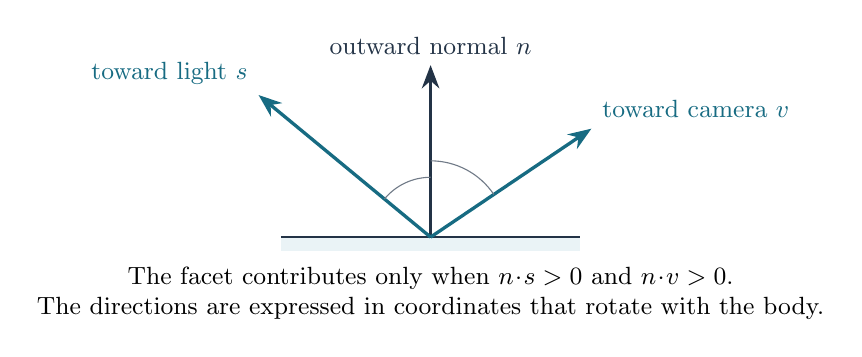
\begin{tikzpicture}[>=Stealth,scale=0.95]
\fill[wash](-2,-.18)rectangle(2,.0);
\draw[thick,ink](-2,0)--(2,0);
\draw[->,very thick,color=ink](0,0)--(0,2.3)node[above,font=\small]{outward normal $n$};
\draw[->,very thick,color=accent](0,0)--(-2.3,1.9)node[above left,font=\small]{toward light $s$};
\draw[->,very thick,color=accent](0,0)--(2.15,1.45)node[above right,font=\small]{toward camera $v$};
\draw[ink!65] (0,.8) arc[start angle=90,end angle=140.4,radius=.8];
\draw[ink!65] (.0,1.02) arc[start angle=90,end angle=34,radius=1.02];
\node[font=\small,align=center] at (0,-.75) {The facet contributes only when $n\!\cdot\!s>0$ and $n\!\cdot\!v>0$.\\The directions are expressed in coordinates that rotate with the body.};
\end{tikzpicture}

\caption{A local view of one facet. The two positive dot products determine illumination and visibility for a convex body. They would not be sufficient for a nonconvex body, where another part of the surface could hide or shadow this facet.}
\end{figure}

Let $\mu_{0}=n\cdot s_{jt}$ and $\mu=n\cdot v_{jt}$. The implemented kernel is
\begin{equation}
 k_{jt}(n)=
 \begin{cases}
 \displaystyle \mu_0\mu\left(100+\frac{1}{\mu_0+\mu+10^{-9}}\right),
       &\mu_0>0\text{ and }\mu>0,\\[4pt]
 0, &\text{otherwise}.
 \end{cases}
 \label{eq:kernel}
\end{equation}
This is a Lambert term with coefficient $100$ plus a Lommel--Seeliger term with coefficient $1$. The small denominator constant avoids numerical division problems. The optional phase-function amplitude and slope are zero. These numbers are a fixed modeling choice; the coefficients are not separately inferred for each object.

For a discrete area measure, unnormalized brightness is the linear sum
\begin{equation}
 B_{jt}(p)=\sum_{i=1}^{N}p_i\,k_{jt}(n_i),
 \qquad f_{jt}(p)=\frac{B_{jt}(p)}{T^{-1}\sum_{u=1}^{T}B_{ju}(p)}.
 \label{eq:brightness}
\end{equation}
An exactly dark predicted curve is represented by zeros. No additive constant is inserted into the mean normalization. Multiplying every physical facet area by the same factor therefore leaves a non-dark normalized curve unchanged. This explains why brightness alone does not set the object's absolute size.

A frozen acquisition calibration shifts each prediction by an angle-dependent integer number of samples and applies a common contrast gain:
\begin{equation}
 \widehat y_{jt}=1+g\bigl(f_{j,t-\Delta_j}-1\bigr),
 \qquad g=0.7349732235818749.
 \label{eq:calibration}
\end{equation}
Indices are circular; the code converts stored shifts in degrees to sample shifts by rounding at the chosen $T$. The stored shifts at measurement angles $0,45,90,135,225,270,315$ degrees are $0,-1,-7,-4,4,7,1$ degrees. They are shared across objects. They came from a separate public-model calibration and are nuisance corrections, not physical estimates of the scattering law.

Weights $w_j$ retain the data-quality policy. In particular, the copied horizontal curve at zero degrees in public Model 3 receives zero weight. Updated Model-1 real curves were used in the September calibration. Simulated curves and public STL shapes are not required by the reconstruction objective.

\clearpage
\section{Representing shape by directional surface area}
A polyhedron has facets with areas $A_i$ and outward normals $n_i$. Its \emph{surface-area measure} places a mass $A_i$ at each normal on the unit sphere. After dividing by total surface area, write
\begin{equation}
 \mu=\sum_i p_i\delta_{n_i},\qquad
 p_i=\frac{A_i}{\sum_r A_r},\qquad \sum_i p_i=1.
 \label{eq:measure}
\end{equation}
Here $\delta_n$ means one unit of mass at direction $n$. A normal is an orientation, not a surface position: the measure is not a cloud of points on the asteroid. ``Gaussian image'' is another name for this directional representation; it does not mean a Gaussian probability density.

\begin{figure}[h]
\centering\resizebox{\linewidth}{!}{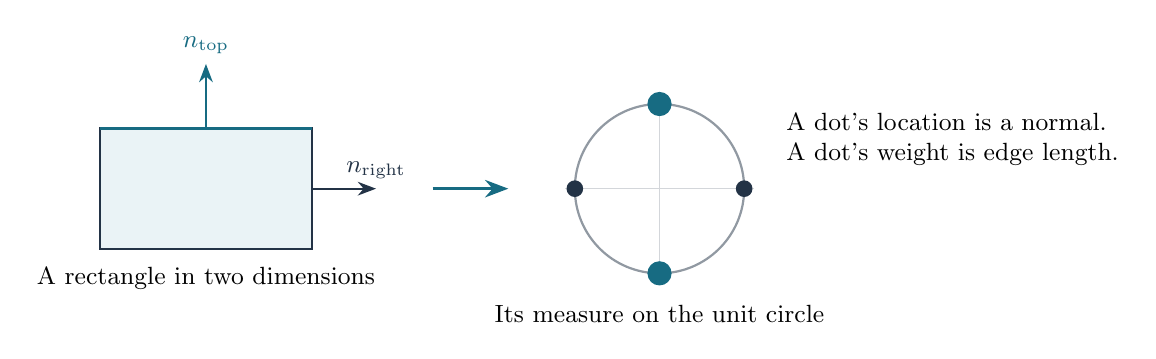
\begin{tikzpicture}[>=Stealth,scale=0.96]
\filldraw[fill=wash,draw=ink,thick] (-1.4,-.8)--(1.4,-.8)--(1.4,.8)--(-1.4,.8)--cycle;
\draw[very thick,color=accent](-1.4,.8)--(1.4,.8);
\draw[->,thick,color=accent](0,.8)--(0,1.65) node[above,font=\small]{$n_{\rm top}$};
\draw[->,thick,color=ink](1.4,0)--(2.25,0) node[above,font=\small]{$n_{\rm right}$};
\node[font=\small] at (0,-1.18) {A rectangle in two dimensions};
\draw[->,very thick,color=accent](3,-.0)--(4,0);
\draw[draw=ink!50,thick](6,0)circle(1.12);
\draw[ink!20] (4.75,0)--(7.25,0) (6,-1.25)--(6,1.25);
\fill[color=accent](6,1.12)circle(.16);
\fill[color=accent](6,-1.12)circle(.16);
\fill[color=ink](4.88,0)circle(.11);
\fill[color=ink](7.12,0)circle(.11);
\node[font=\small,align=left,anchor=west] at (7.55,.65) {A dot's location is a normal.\\A dot's weight is edge length.};
\node[font=\small] at (6,-1.65) {Its measure on the unit circle};
\end{tikzpicture}
}
\caption{A two-dimensional analogy. Opposite long edges create larger, opposite masses on the unit circle. In three dimensions, facet areas replace edge lengths and the unit sphere replaces the circle. This illustration is schematic, not a recovered challenge shape.}
\end{figure}

A necessary balance condition for a closed surface is
\begin{equation}
 \sum_i p_i n_i=0.\label{eq:closure}
\end{equation}
It follows from the divergence theorem applied to constant vector fields: a closed surface has zero net oriented area. For positive masses whose normals span three dimensions, this condition also underlies Minkowski's existence and uniqueness theorem: the areas and normals determine a convex polyhedron up to translation~\cite{sellaroli2017}. Unit total area fixes its scale before the final challenge-frame transformation.

\subsection*{A positive chart with only 45 shape coefficients}
The dense fitting stage uses $N=512$ directions from the established spherical quadrature grid. A real spherical harmonic is an oscillating function on the sphere, analogous to a Fourier mode on a circle. Degrees $2$ through $6$ give $45$ active coefficients. With centered and normalized basis functions $Y_r$,
\begin{equation}
 \ell_i=\sum_{r=1}^{45}c_r Y_r(n_i),\qquad
 p_i(c)=\frac{q_i\exp\bigl(\ell_i+b(c)\cdot n_i\bigr)}
 {\sum_r q_r\exp\bigl(\ell_r+b(c)\cdot n_r\bigr)}.
 \label{eq:chart}
\end{equation}
Here $q_i$ are positive reference weights for the bounding spheroid, defined on the next page. The exponential guarantees positivity and the denominator fixes total mass. For each $c$, a three-variable solve finds $b(c)\in\R^3$ so that~\eqref{eq:closure} holds to numerical tolerance. Equivalently, it minimizes the convex log-partition function in $b$; its gradient is the closure vector and its Hessian is the normal covariance. Derivatives through this solve preserve the linearized constraints.

Degree zero is redundant with mass normalization, while the three degree-one modes are supplied by the closure tilt. The phrase ``Bayes--Hilbert'' in the code refers to this log-density representation. The chosen objective below uses an OT surface prior; its separate surface log-density penalty is switched off.

\clearpage
\section{Fitting the measure with an optimal-transport prior}
The reference $q$ is the surface-area distribution of an axis-aligned spheroid with semiaxes $(R,R,1)$, sampled on the same normal grid. If $\omega_i$ is a spherical quadrature weight, then
\begin{equation}
 q_i\ \propto\ \omega_i\,
 \frac{R^4}{\left[R^2(n_{ix}^2+n_{iy}^2)+n_{iz}^2\right]^2},
 \qquad \sum_i q_i=1.\label{eq:reference}
\end{equation}
This uses only the released radius. It is a preference for a broad aspect ratio, not a claim that the unknown object is a spheroid.

\subsection*{Moving mass between nearby directions should be inexpensive}
A pointwise penalty compares masses only at identical grid locations. Optimal transport instead asks how much mass must move, and how far, to turn one distribution into another. For unit directions we use squared \emph{chordal} distance,
\begin{equation}
 C_{ir}=\norm{n_i-n_r}^{2}=2-2n_i\cdot n_r.
\end{equation}
It measures straight-line distance in $\R^3$ between points on the sphere, rather than great-circle distance.

For two probability vectors $a,b$, the entropy-regularized transport problem is
\begin{equation}
 \OT_\varepsilon(a,b)=\min_{\substack{\pi\geq0\\\pi\mathbf1=a,\ \pi^\top\mathbf1=b}}
 \left\{\sum_{ir}\pi_{ir}C_{ir}
 +\varepsilon\sum_{ir}\pi_{ir}\log\frac{\pi_{ir}}{a_i b_r}\right\}.
 \label{eq:ot}
\end{equation}
The matrix $\pi$ specifies the amount sent from each source direction to each destination. Entropy regularization makes this transport plan less concentrated and allows matrix-scaling iterations~\cite{cuturi2013}. We use $\varepsilon=0.05$ and $200$ Sinkhorn iterations. The result is a differentiable finite-iteration approximation, with marginal residuals recorded.

The self-cost is removed using the Sinkhorn divergence~\cite{feydy2019}:
\begin{equation}
 S_\varepsilon(p,q)=\OT_\varepsilon(p,q)
 -\tfrac12\OT_\varepsilon(p,p)-\tfrac12\OT_\varepsilon(q,q).
 \label{eq:sinkhorn}
\end{equation}
Thus the prior has zero value at its own reference. It approximates a squared transport distance; we do not identify the finite-iteration quantity with an exact Wasserstein distance.

\subsection*{The actual objective}
Let $M(p)=\sum_i p_i n_i n_i^\top$ be the second normal moment. Its trace is one; its entries describe broad directional anisotropy. The fitted objective is exactly
\begin{equation}
 \mathcal J(c)=
 \underbrace{\frac{\sum_j w_j\sum_t(\widehat y_{jt}(p(c))-y_{jt})^2}
 {2T\sum_j w_j}}_{\text{brightness residual}}
 +\frac{\lambda_W}{2}S_\varepsilon(p(c),q)
 +\frac{0.2}{2}\norm{M(p(c))-M(q)}_F^2.
 \label{eq:objective}
\end{equation}
The last term controls a weakly constrained large-scale aspect mode. Other available penalties have zero coefficients. Each fit uses three deterministic starts, $300$ Adam steps and up to $100$ L-BFGS iterations. The base seed is $20260820$, plus the model identifier. The objective and its diagnostics, rather than any known shape, choose the dense fitted endpoint.

\clearpage
\section{Turning a dense measure into a small set of facets}
Directly realizing hundreds of tiny facet masses can be poorly conditioned. The next stage compresses the fitted measure into at most $K$ directions while preserving the balance required for a closed body.

For sites $u_1,\ldots,u_K\in\sphere$, the free-weight quantization objective is
\begin{equation}
 Q(u_1,\ldots,u_K)=\sum_i p_i\min_k\frac12\norm{n_i-u_k}^2.
 \label{eq:quantization}
\end{equation}
The implementation alternates two steps. First assign every input direction to its nearest site, producing cells $C_k$. Then move each site to the normalized weighted resultant of its assigned directions:
\begin{equation}
 r_k=\sum_{i\in C_k}p_i n_i,\qquad u_k=\frac{r_k}{\norm{r_k}}.
 \label{eq:resultant}
\end{equation}
This is weighted spherical Lloyd iteration. The code calls the stage semidiscrete OT quantization; both the fitted source and the emitted output are represented discretely. Eight restarts include a deterministic Ward initialization: hierarchical grouping of nearby directions. A fixed seed, up to $200$ iterations, and a declared convergence tolerance make the procedure reproducible. Lloyd iteration finds a local solution, not a globally optimal partition.

\subsection*{The important correction: cell mass is not facet area}
An ordinary quantizer would give site $k$ its cell mass $s_k=\sum_{i\in C_k}p_i$. In general $\sum_k s_k u_k\ne0$, so these weights would not describe a closed polyhedron. We instead emit
\begin{equation}
 a_k=\frac{\norm{r_k}}{\sum_l\norm{r_l}},\qquad
 \nu=\sum_k a_k\delta_{u_k}.
 \label{eq:emitted}
\end{equation}
Closure is preserved algebraically:
\begin{equation}
 \sum_k a_k u_k
 =\frac{\sum_k r_k}{\sum_l\norm{r_l}}
 =\frac{\sum_i p_i n_i}{\sum_l\norm{r_l}}=0.
 \label{eq:resultantclosure}
\end{equation}
The resultant length is smaller when the cell contains a wide spread of directions. Consequently, $a_k$ need not equal $s_k$. The original nearest-site transport plan is a plan to the cell-mass measure, not to the corrected measure $\nu$.

To account for this distinction, each restart's \emph{emitted} measure is scored by a separate exact discrete transport linear program with the full squared chordal cost. The best valid restart is retained using that score, rather than merely its Lloyd objective.

\subsection*{A mass floor preserves numerical realizability}
After restart selection, any emitted mass below $10^{-8}$ is merged with a partner chosen to minimize the increase in the spherical Ward objective. Adding the two resultants preserves their sum and therefore preserves closure. Masses are renormalized and the check is repeated. This is a deterministic merge rule, not a globally solved mass-constrained transport problem.

The effective number of directions can be smaller than the requested $K$. Every merge and its transport change is recorded. We do not subsequently move the sparse normals or refit their masses in this submission method. Zero resultants or invalid geometric configurations cause a recorded failure rather than an unchecked mesh.

\clearpage
\section{Building the polyhedron and placing it in the challenge frame}
After quantization the normals $u_k$ and positive areas $a_k$ are fixed. The remaining unknowns are plane positions, represented by support numbers $h_k$:
\begin{equation}
 P(h)=\{x\in\R^3:u_k\cdot x\leq h_k\text{ for all }k\}.
 \label{eq:polytope}
\end{equation}
The facet at $u_k\cdot x=h_k$ must have area $a_k$. The normal-span and closure conditions ensure that this is the appropriate Minkowski reconstruction problem~\cite{sellaroli2017}.

\subsection*{Why volume leads to the right facet areas}
Moving one plane outward by a small distance adds a thin slab of volume. Therefore
\begin{equation}
 \frac{\partial V(h)}{\partial h_k}=A_k(h),
 \label{eq:volumederivative}
\end{equation}
where $A_k(h)$ is the area of facet $k$. The variational problem of maximizing $V(h)$ with $\sum_k a_kh_k$ fixed has stationarity equations $A_k(h)=\eta a_k$. A final uniform scale removes $\eta$.

The implementation solves the prescribed-area equations with damped Newton continuation, beginning with an equal-support polytope. It uses analytic derivatives of facet area with respect to adjacent support numbers. Translation is a three-dimensional nullspace: replacing $h_k$ by $h_k+u_k\cdot t$ translates the body by $t$. Newton steps fix this freedom, and the realized body is finally centered at its volume centroid.

Every prescribed positive atom must remain an active facet. The strict tolerance is $10^{-6}$ for root-mean-square log-area error. The solver also checks closure, positivity, active facets, orientation, and volume identities. It does not discard inconvenient atoms or add an artificial closing facet.

\subsection*{Size normalization changes the directional measure}
The challenge convention is applied after realization: translate only in $z$ to center the vertical extrema, scale uniformly to make the height two, and scale $x,y$ together about the fixed origin to match $R$. There is no new horizontal centering or phase-fitting rotation. In general the linear part is anisotropic,
\begin{equation}
 L=\diag(s\rho,s\rho,s),\qquad s>0,\quad\rho>0.
\end{equation}
Anisotropic scaling changes both normals and relative facet areas. The oriented area vectors transform by the cofactor matrix:
\begin{equation}
 b_k=\cof(L)(a_ku_k),\quad
 \cof(L)=\det(L)L^{-\top},\quad
 u'_k=\frac{b_k}{\norm{b_k}},\quad
 a'_k=\frac{\norm{b_k}}{\sum_l\norm{b_l}}.
 \label{eq:cofactor}
\end{equation}
Because this map is linear on area vectors, it preserves closure. Brightness is then recomputed from $(a'_k,u'_k)$ and independently from the triangles read back from the exported STL. Their maximum prediction difference must be at most $10^{-5}$. The export also checks a closed, consistently oriented mesh, positive volume, vertical contacts, and cylinder containment/contact. This replay verifies what is delivered; the earlier dense-fit residual alone cannot do so.

\clearpage
\section{Parameter selection and public calibration}
This release uses one shared preset, $\lambda_W=0.03$ and requested $K=64$, with the $10^{-8}$ mass floor. The prior strength controls the fitted dense distribution; the facet count controls its sparse geometric realization.

Choosing parameters per object from its observed data is allowed. We tested a fixed L-curve rule that seeks a bend in data error versus regularization or complexity. A nonmonotone Model-2 path and nearly straight Model-1/3 complexity curves made this choice unreliable; public performance did not improve. This bounded trial supports retaining the shared preset for this release.


\subsection*{What the released evaluation code measures}
Our September calibration used the organizers' unchanged Python voxel evaluator and native MATLAB projection metric. We report $1-\text{Dice loss}$ and retain Python's two real padding cubes. MATLAB separately centers each mesh by its vertex mean, rotates about $z$, and compares its XY projected outline. Its angle changes the top-view raster orientation, not the viewing direction.

We used voxel pitch $0.05$, MATLAB angle $0$ degrees, and the sum of the positive voxel and projection scores. This follows the released examples, but does not establish the organizers' eventual leaderboard settings. Native target caching was required to agree bit for bit with the unmodified MATLAB function.

\begin{table}[h]
\centering
\begin{tabular}{@{}lrrrr@{}}\toprule
Public model & Effective facets & Voxel & Projection & Total (max. 2) \\\midrule
1 & 64 & 0.962625 & 0.991082 & 1.953707 \\
2 & 45 & 0.894000 & 0.967597 & 1.861597 \\
3 & 64 & 0.726896 & 0.950645 & 1.677542 \\\midrule
Equal-model mean & --- & 0.861174 & 0.969775 & 1.830949 \\
\bottomrule\end{tabular}
\caption{Public results for the shared calibration setting $\lambda_W=0.03$, requested $K=64$, and mass floor $10^{-8}$. These numbers describe this setting; they are not secret-model accuracy estimates.}
\end{table}

The shared setting was the best of a predeclared grid with $\lambda_W\in\{0.03,0.1,0.3,1\}$ and $K\in\{7,16,32,64\}$: $48$ public candidates, all geometrically valid. It lies at the lowest tested regularization and highest tested facet count. The runner-up, $(0.3,64)$, had mean combined score $1.819112$. Reevaluation of those two settings at pitch $0.025$ and raster angle $45$ degrees preserved their mean ordering: $1.829689$ versus $1.818346$. No grid expansion followed those scores.

Omitting each public model in turn changed the setting selected on the other two in two of three folds. Model 3 has the weakest volume overlap; Model 2 retains a substantial brightness residual. Transfer of parameter choices remains uncertain, and the method cannot recover nonconvex detail.

\clearpage
\section{Reproducibility and numerical checks}
The accompanying repository contains the production reconstruction code and configuration. It records input-file hashes, the selected parameters, seeds, geometric diagnostics, final-frame residuals, and exported STL hashes. The public geometry evaluator is a calibration tool; reconstruction can run from the lightcurve tables, their acquisition metadata, and the released radius without reading a target shape.

The following checks have different purposes and should not be conflated:
\begin{itemize}
\item \textbf{Data-fit checks} measure agreement with the available brightness curves under the assumed scattering model.
\item \textbf{Realization checks} establish that the chosen positive, balanced measure was converted into the intended closed convex mesh.
\item \textbf{Export replay checks} establish that the serialized STL and the transformed measure predict the same brightness.
\item \textbf{Public shape scores} assess geometric accuracy where a reference shape is available. They are calibration evidence, not a theorem about the secret objects.
\end{itemize}

The STL also receives a numerical convex-boundary certificate: its triangles must cover the outward boundary of their convex hull once. This combines topology, supporting-plane, area and volume checks, with relative tolerances of $10^{-7}$ (plane distances scaled by the bounding-box diagonal). It is not a generic exact intersection test; sub-tolerance defects remain unresolved.

\subsection*{Limitations of the construction}
Convex visibility cannot describe remote self-shadowing or a hidden concavity. Calibration corrections can absorb discrepancies without identifying their geometric cause. Finite multistart fitting, Lloyd iteration, and entropic transport approximations provide numerical candidates and explicit diagnostics, rather than global or statistical guarantees.

\vspace{3pt}
{\small
\bibliographystyle{plainnat}
\bibliography{references}
}
\end{document}
